\chapter{Head Pose Estimation}
\label{sec:HPestimation}
Efficient and accurate head pose estimation can be very useful to many application, but it is a very challenging problem. By using the approach proposed by Fanelli \cite{GFRF}, accurate pose estimation is achieved. Random regression forest is the algorithm of choice since its ability to handle big datasets. In this chapter, I will discuss the training procedure of such forest in detail in \ref{sec:RFtraining}. The evaluation is done on a synthetic dataset of 3D images. And the performance of such forest will be discuss in \ref{sec:HPevaluation}.


\clearpage
\section{Random Forest Training}
\label{sec:RFtraining}
A tree in the forest is trained from annotated patches randomly extracted from a subset of the training images. Each tree is assigned a maximum depth which it is allowed to grow to. The depth of the trees is relative to the performance of the forest during the testing time. Beginning at the root, every tree is build recursively by applying binary test at each non-leaf node. These tests will decide which direction will each patch be sent. i.e. left or right child of that node. Binary tests used are also randomly selected from a test pool. There is a trade-off between how many tests to be done at each node and how much time to be spent at each node. Generally the more tests to be done the more accurate split will be achieved. The goal of all the binary test is to find best one that maximizes the information gain. \cite{GFRF} The problem is essentially an optimisation problem. Analytically, the objective function is: 
\begin{equation}
\label{eq:argmax}
\theta ^* = \arg \max\limits_{\substack{ \theta}} IG(\theta)
\end{equation}

\begin{equation}
\label{eq:diffentropy}
IG(\theta) = H(P) - \sum\limits_{i \in \{ left,right \}} w_{i} H(P_{i}(\theta))
\end{equation}

Where $w_{i} =  \frac{|P_{i}(\theta)|}{|P|}$ which is the proportion of patches each child has after every split. $H(P)$ is the entropy measurement. (discussed in \ref{subsec:measureofentropy}) This process will continue until the maximum depth is reached. Once the maximum depth is reached, the nodes are classified as leaf nodes and necessary information will be store at such nodes.

\subsection{Training Data}
\label{subsec:HPdataset}
Training data is depth images annotated with the 3D locations of the tip of the nose together with the three head rotational angles, namely pitch, yaw, roll. Square patches with fixed size are extracted from each depth image. Each patch is annotated with two vectors: $\alpha ^{1} = (\alpha _{x}, \alpha _{y}, \alpha _{z} )$ is the 3D offset vector between the centre of the patch and the position of the nose. And $\alpha ^{2} = (\alpha _{pitch}, \alpha _{yaw}, \alpha _{roll} )$ is the head orientation as Euler angles. Since when patches are sampled, they are sampled not only from the face but also from other body parts like torso. Every patch is also given a class label $c_{i} \in \{1,0\} $ as positive (near the face) or negative (far from face) respectively. As a result, each training patch is therefore in the form of $P_{i} = (I_{i},c_{i}, \alpha ^{1}, \alpha ^{2}) $ Where $I_{i}$ is the feature obtained from each patch, in this case it is the original depth values. \cite{GFRF}

\subsection{BinaryTest At Non leaf nodes}
\label{subsec:binarytest}
The binary test at each node is defined as follows:
\begin{equation}
\label{eq:binarytest}
|F_{1}|^{-1} \sum\limits_{q \in F_{1}} I(q) - |F_{2}|^{-1} \sum\limits_{q \in F_{2}} I(q) > \tau
\end{equation}
Where $F_{1} $ and $F_{2}$ is two rectangles  within the patch and $\tau$ is a threshold. What the above equation essentially represents is the difference between the average values of two rectangles which is very similar to the Haar-like feature mentioned in \ref{sec:HLfeatures}. \cite{GFRF} As shown in Figure \ref{fig:patch}. All the best tests found will be store at every non-leaf node.

\begin{figure}
	\centering
	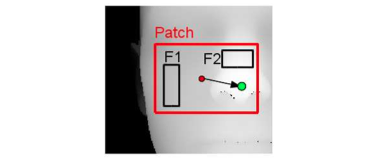
\includegraphics[width=0.8\linewidth]{patch.png}
	\caption[sample patch]{\label{fig:patch}}  \textbf{Example of a training patch (the red box), rectangles F1,F2 are randomly chosen within the patch, red dot is the patch centre and the green dot is the location of the nose } \cite{GFRF}
\end{figure}

\subsection{Measure of Entropy}
\label{subsec:measureofentropy}
At each node, vectors $\alpha ^{1}, \alpha ^{2}$ can be modelled as realisations of multivariate normal random variable. \cite{DRFHP} And by definition, the differential entropy for a random variable is: 
\begin{equation}
\label{eq:diffentropy}
h(x) = -\int_X f(x) log f(x) dx 
\end{equation}
 The probability density function for a k-dimensional normal is :
\begin{equation}
\label{eq:mvnormal}
f_{\textbf{x}}(x_{1}, , ,x_{k}) = \frac{1}{\sqrt{(2\pi)^{k}|\mathbf{\Sigma}|}}exp(- \frac{1}{2}(\mathbf{x}-\mu)^{T}\mathbf{\Sigma}^{-1}(\mathbf{x}-\mu))
\end{equation}
Applying both above equations with k = 3, we find the differential entropy is :
\begin{equation}
\label{eq:df1}
H(P)^{n} = \frac{1}{2}log((2\pi e)^{3}|\mathbf{\Sigma}^{n}|)
\end{equation}
where $ n \in (1,2)$ . However, from equation \refeq{eq:df1}, we can deduce the regression measure is:
\begin{equation}
\label{eq:rm1}
H_{r}(P) = \sum\limits_{n}log(|\mathbf{\Sigma}^{n}|) \propto H(P)^{n}
\end{equation} 
Now we can substitute equation \refeq{eq:rm1} into \refeq{eq:diffentropy}, maximising equation \refeq{eq:diffentropy} favours binary tests chosen earlier which minimize the determinant of the covariance matrix $\mathbf{\Sigma} $and reduces the regression uncertainty. \cite{GFRF,DRFHP}

At testing time, once a patch is passed down to the forest, the forest is used not only to give probabilistic votes in a continuous space but also to determined the patch is eligible to cast a vote. Therefore a measure of the classification uncertainty at training time is needed in this case. \cite{GFRF,DRFHP}
\begin{equation}
\label{eq:cumeasure}
H_{c}(P) = - \sum\limits_{k=0}^K p(c=k|P)log(p(c=k|P))
\end{equation}
Where K = 1 meaning the patch is either positive or negative.  Now we have two measures \refeq{eq:rm1} and \refeq{eq:cumeasure} and we combine them as a weighted sum of two as proposed by Okada \cite{okada,GFRF}:
\begin{equation}
\label{eq:okada}
H_{c}(P) + \alpha max(p(c=1|P)-t_{p},0)H_{r}(P)
\end{equation}
When minimising the above, the second term is zero until the proportion of the positive patches reaches a threshold. Then the second term comes into play. The choices of $t_{p}, \alpha$ will be mentioned in \ref{sec:HPevaluation}

\subsection{Information to be stored at leaves}
\label{subsec:leafdistribution}
Once the patches get to the maximum depth, leaf nodes will be formed and few bits of information will be stored. Firstly, since patches are mark as positive or negative at the early stage, the percentage of positive patches reach at the leaves is recorded which is essentially the class probability $p(c=k|P)$. And the mean vectors and traces of the covariance matrices computed from $\alpha ^{1}$  and $\alpha ^{2}$ of all the patches arrived at each leaf node. In this way, a combination of classification and regression forest is built ready for the experiments.

\clearpage
\newpage
\thispagestyle{plain}
\mbox{}
\section{Evaluation}
\label{sec:HPevaluation}

\subsection{Dataset}
\label{subsec:hpdataset}
The experiment is conducted on Biwi Kinect Head Pose Database which is a synthetic database and contains over 15000 images capture from 20 people, all of which are annotated with the 3D nose position, the head rotation angles and have resolution $640 \times 480$ . The yaw, pitch and roll angle are within the range of $\pm75 \pm60 \pm50 $ respectively. Each depth image contains not only the head but the other body parts with the background removed ( value of each pixel that does not belong to the person will be zero). Head mask which can be used to sample positive patches are also provided. \cite{GFRF} 

\subsection{Experiments}
\label{subsec:experiment}
As far as training is concerned, image 15 subjects out of 20 are used and the remaining 5 people are used for testing. In the For each tree, 2000 images are randomly sampled from the image pool. For each image, 40 patches are sampled , 20 positive and 20 negative patches as shown in Fig \ref{fig:patchi}. Positive patches are sample using the masks as shown in Fig \ref{fig:headmask}. Negative patches are sample from other  body parts. 

\begin{figure}
	\centering
	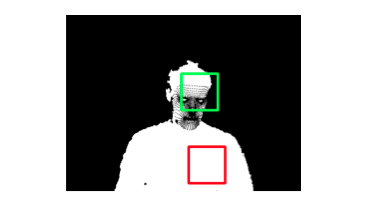
\includegraphics[width=0.8\linewidth]{patchesimage.png}
	\caption[depth image with positive and negative patches]{\label{fig:patchi}}  \textbf{positive patch in green, negative patch in red } \cite{GFRF}
\end{figure}

Every patch occupies an area of $80 \times 80 $ pixels. When growing each tree, maximum depth is set to 15 and at non-leaf nodes, 500 random pairs of rectangles $F_{1}, F_{2}$ in Fig \ref{fig:patch} and 20 random thresholds in equation \refeq{eq:binarytest} are selected from the pool. Therefore in total 10000 tests are carried out for each incoming training patch at each non-leaf node. If the number goes beyond this threshold the training time takes too long and the performance does not scale very much. As mentioned in \ref{subsec:measureofentropy}, parameters $\alpha, t_{p}$ are set to 1.0 and 0.7 as suggested by \cite{okada}.

\begin{figure}
	\centering
	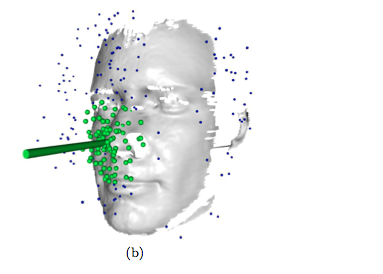
\includegraphics[width=0.5\linewidth]{outliers.png}
	\caption[outliers]{\label{fig:outliers}}  \textbf{blue dots are the outliers and green dots are the votes used to give the actual estimated } \cite{GFRF}
\end{figure}

\begin{figure}
	\centering
	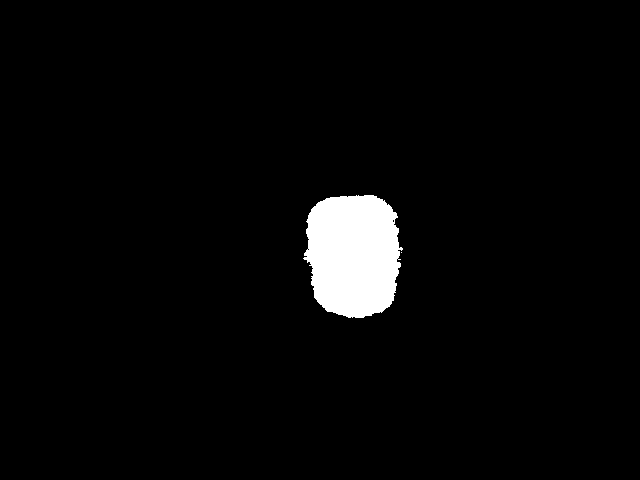
\includegraphics[width=0.8\linewidth]{frame_00004_depth_mask.png}
	\caption[Head mask used to select positive patch]{\label{fig:headmask}}  \textbf{White pixel area represents the head position, positive patches will be sampled around this area } 
\end{figure}

During the testing time as illustrated in Fig \ref{fig:rftest}, since the data is provided with the background removed, bounding boxes around the actual data are extracted first from test images and patches are sampled within such bounding boxes. Each patch is passed down the tree and then directed by the binary test store during the training until it reaches a leaf node where the patch centre in 3D representation will be added onto the mean 3D offset vector stored at leaf node earlier to give an estimated of the nose position. Integral image is used when computing the binary tests therefore extra computation time is ignored. 

A patch is allowed to cast a vote only if the positive class probability at that leaf node is 1 and the trace of the covariance matrix of the nose position is below a threshold. Since leaf nodes with high variance at the nose position are not informative and will affect the result. The lower the threshold is ,the more votes will be filtered before the final estimation which could speed up the estimation process and decrease the uncertainty of the estimation.The threshold of the trace of the covariance matrix is set from 300 to 2000 to observe the corresponding performance and plots are shown in Fig \ref{fig:accuracyvstrace}. As we can see from the plot, overall accuracy decreases as the maximum variance allowed for a patch to cast a vote and the good accuracy is achieved around 400.

\begin{figure}
	\centering
	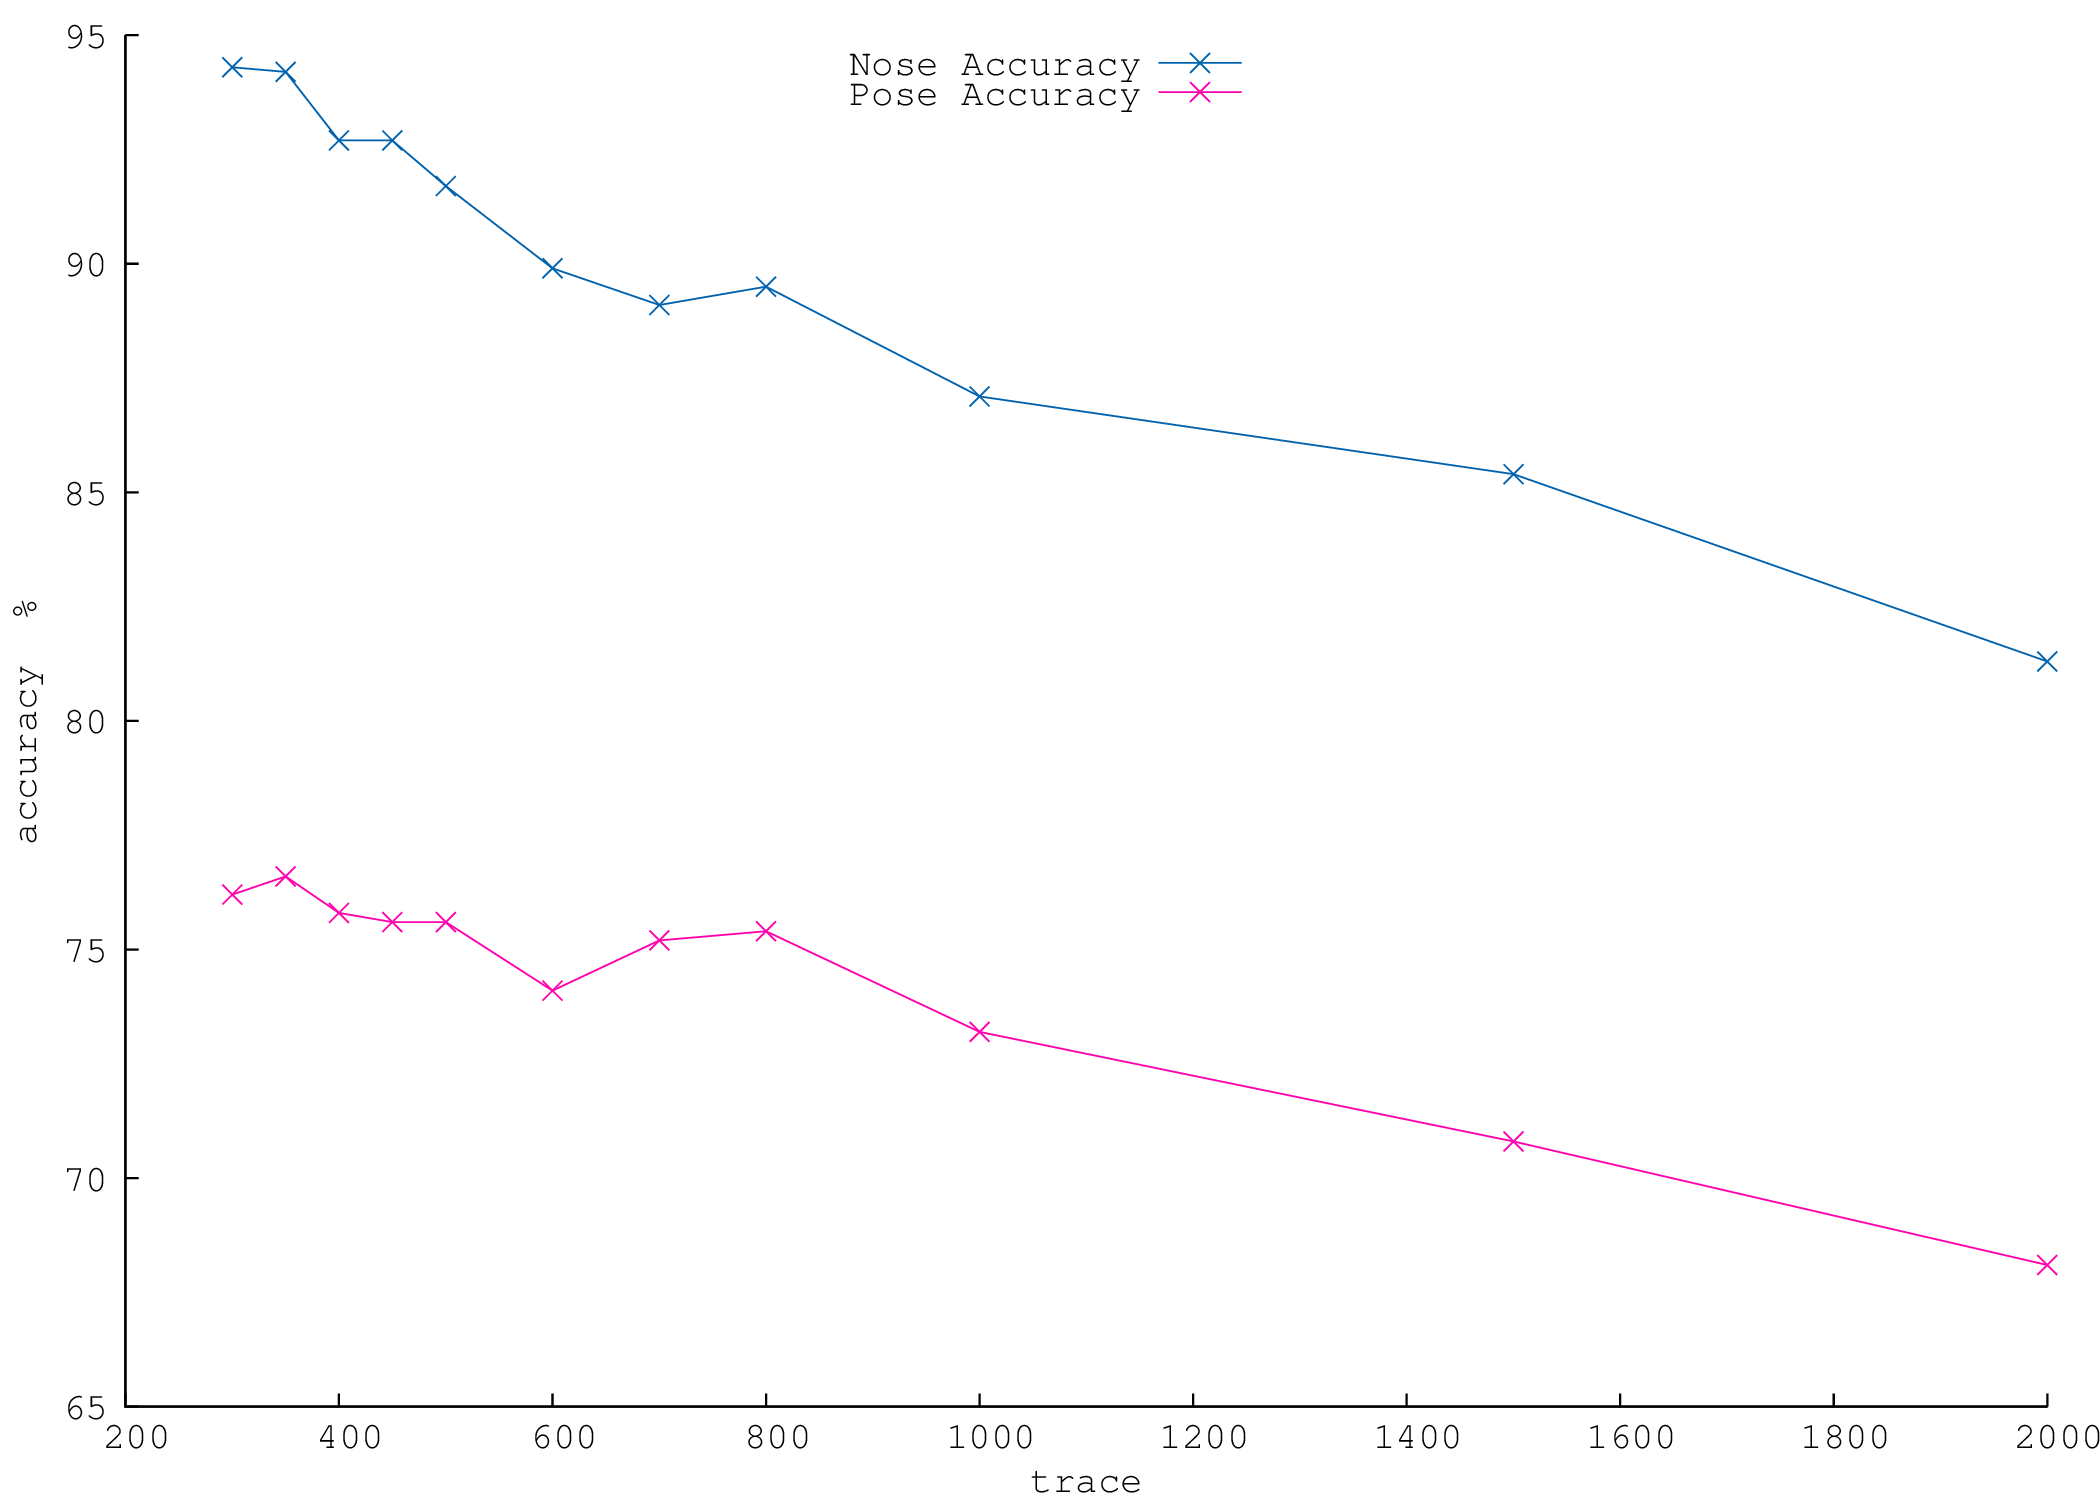
\includegraphics[width=0.8\linewidth]{accuracyvstrace.png}
	\caption[Accuracy vs trace]{\label{fig:accuracyvstrace}}  \textbf{Accuracy for nose and pose estimation vs maximum variance, nose in pink and pose in blue} 
\end{figure}

 After every test patch is processed, there is a huge pool of candidate votes and there will be outliers. (see in fig \ref{fig:outliers}) And it turned out to be essential to remove these outliers before moving on to the next step. These outliers are removed by mean shift. \cite{GFRF} Then the mean of the remaining votes is computed again to be the final estimated.

How densely the test patches will be sample will directly affect the result as well. There is a tradeoff between how much time to be spent and how much accuracy to get.  In this case, since the synthetic data is with the background removed, patches only needs to be sampled within the window that covers the person's body but not the whole image. Where the accuracy denotes the success rate among test images. A successful detection is achieve if the nose error is below 20mm and the angle error is below 15 degrees. \cite{GFRF}


The accuracy for both nose the angles are plotted in figure \ref{fig:avt}.The test is performed on 500 test images with various density that patches are sampled.As can be seen from the plots, number of trees loaded for the estimation affect the result more in the early stage but as more trees are loaded, the performance improves in a more gradual manner and finally converges. And as more patches are sample for each test image, the accuracy could improve from 70\% to almost 90\%.


\begin{figure}
	\centering
	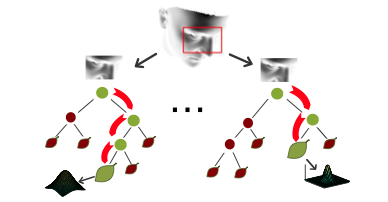
\includegraphics[width=0.8\linewidth]{randomforest.png}
	\caption[testing time forest]{\label{fig:rftest}}  \textbf{testing patches are passed down to each tree to get a possible vote at the arrived leaf node \cite{GFRF}} 
\end{figure}


\begin{figure}
        \centering
	 \begin{subfigure}[b]{0.5\textwidth}
                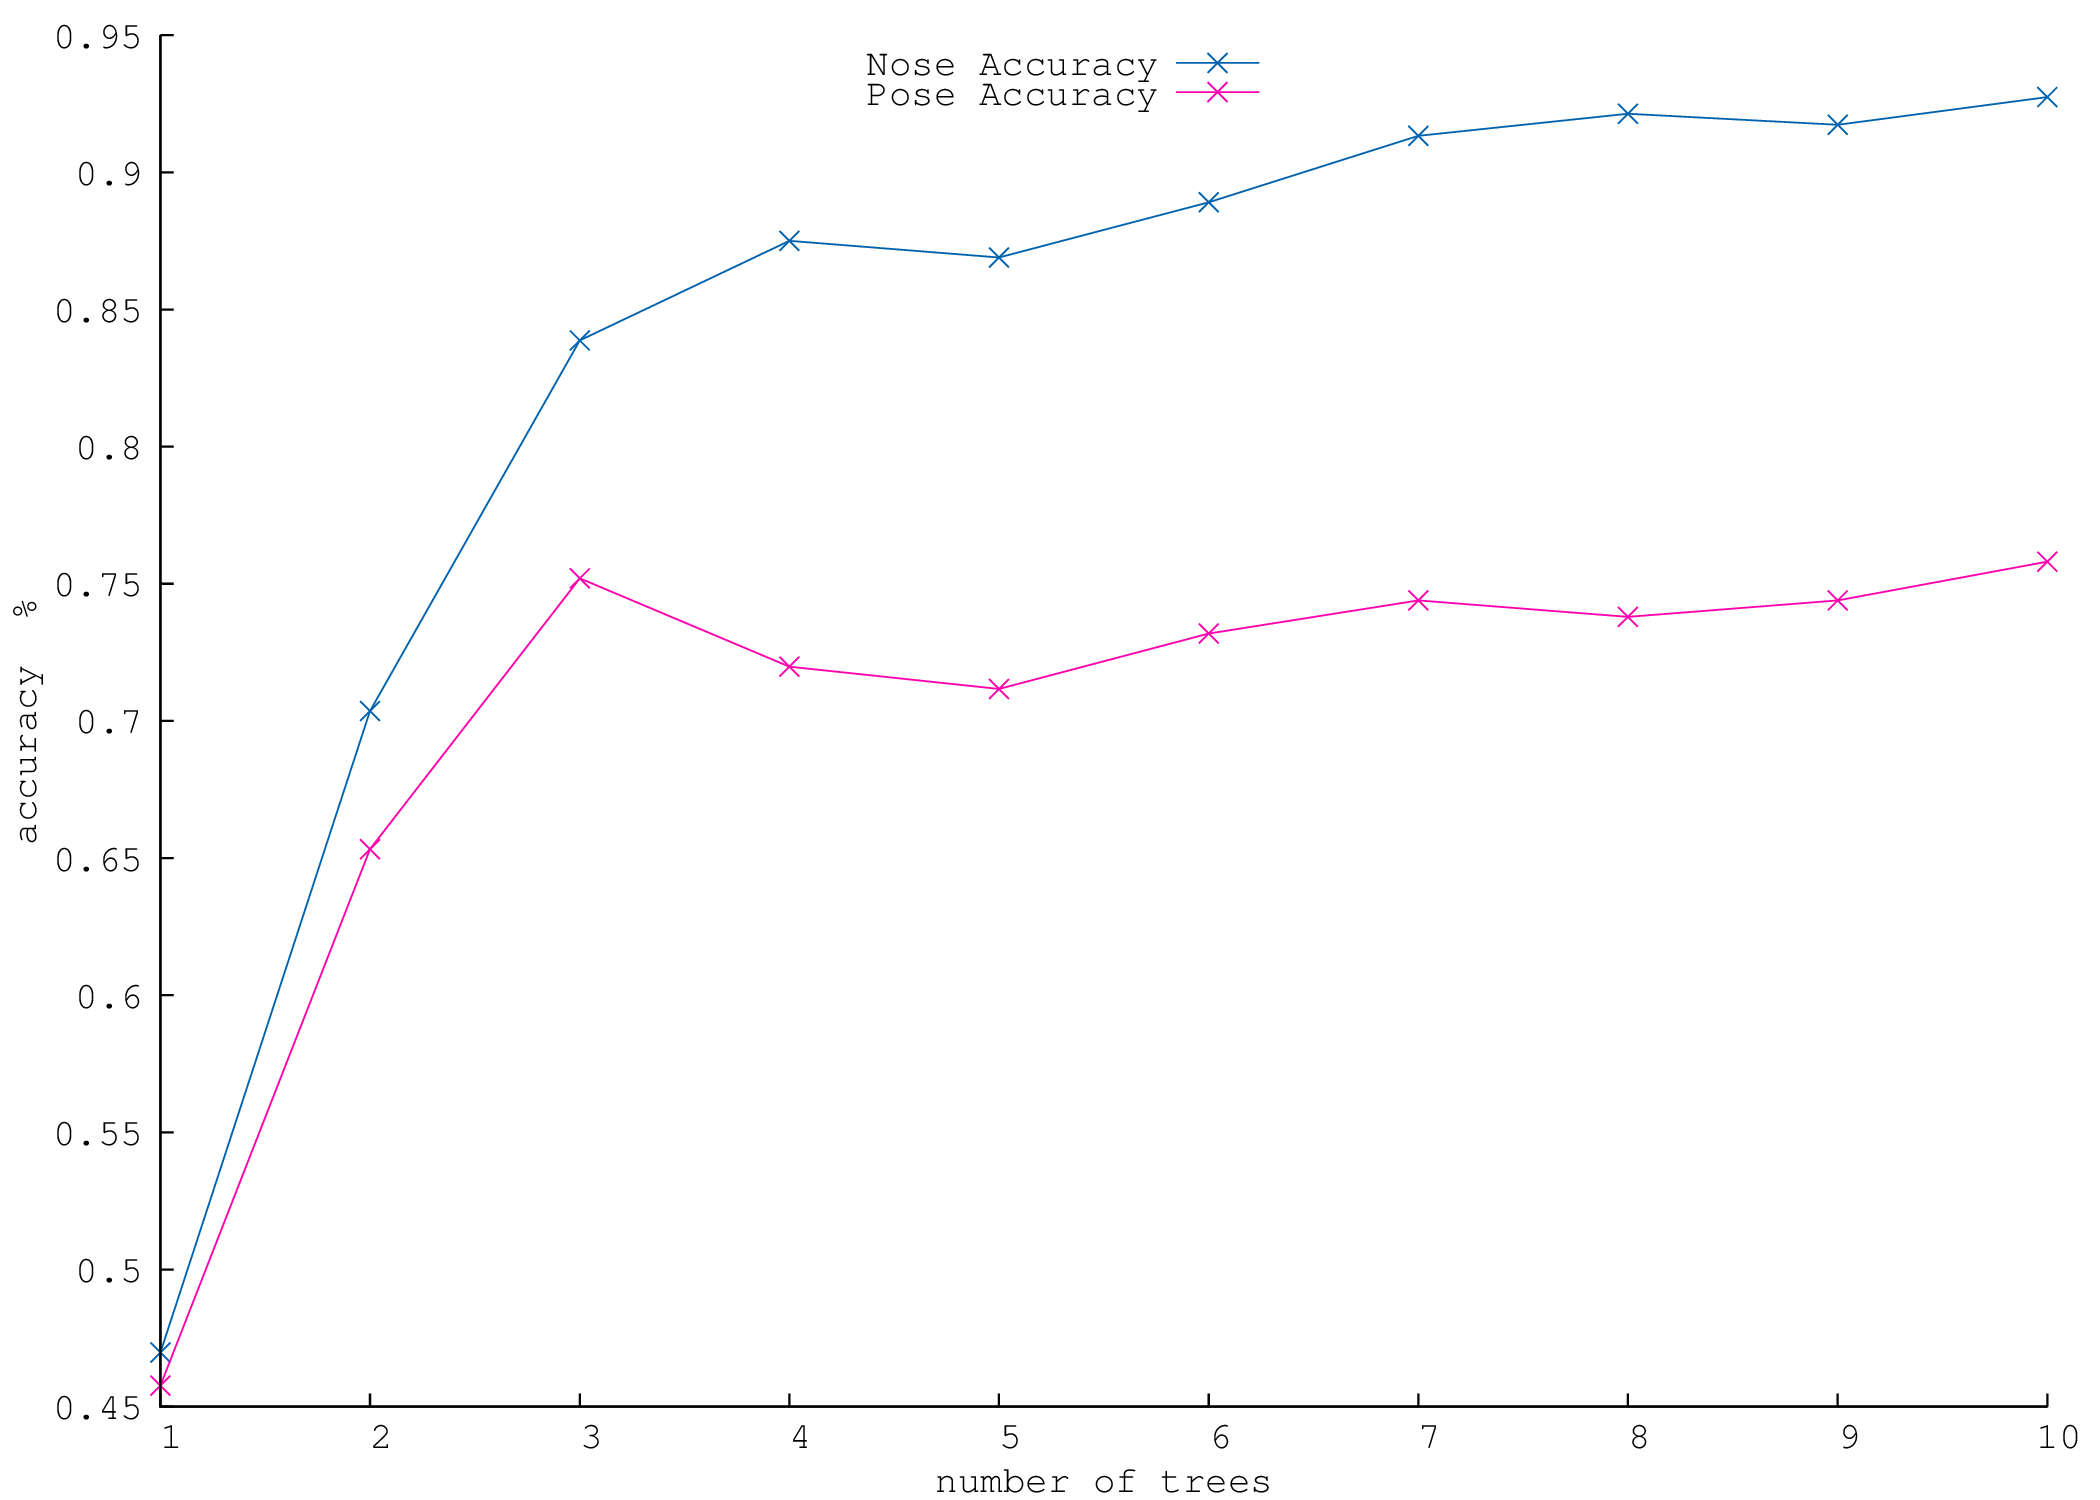
\includegraphics[width=\textwidth]{3daccuracyvstreesstepsize5.png}
                \caption{stride 5}
                \label{fig:naa5}
        \end{subfigure}%
        \begin{subfigure}[b]{0.5\textwidth}
                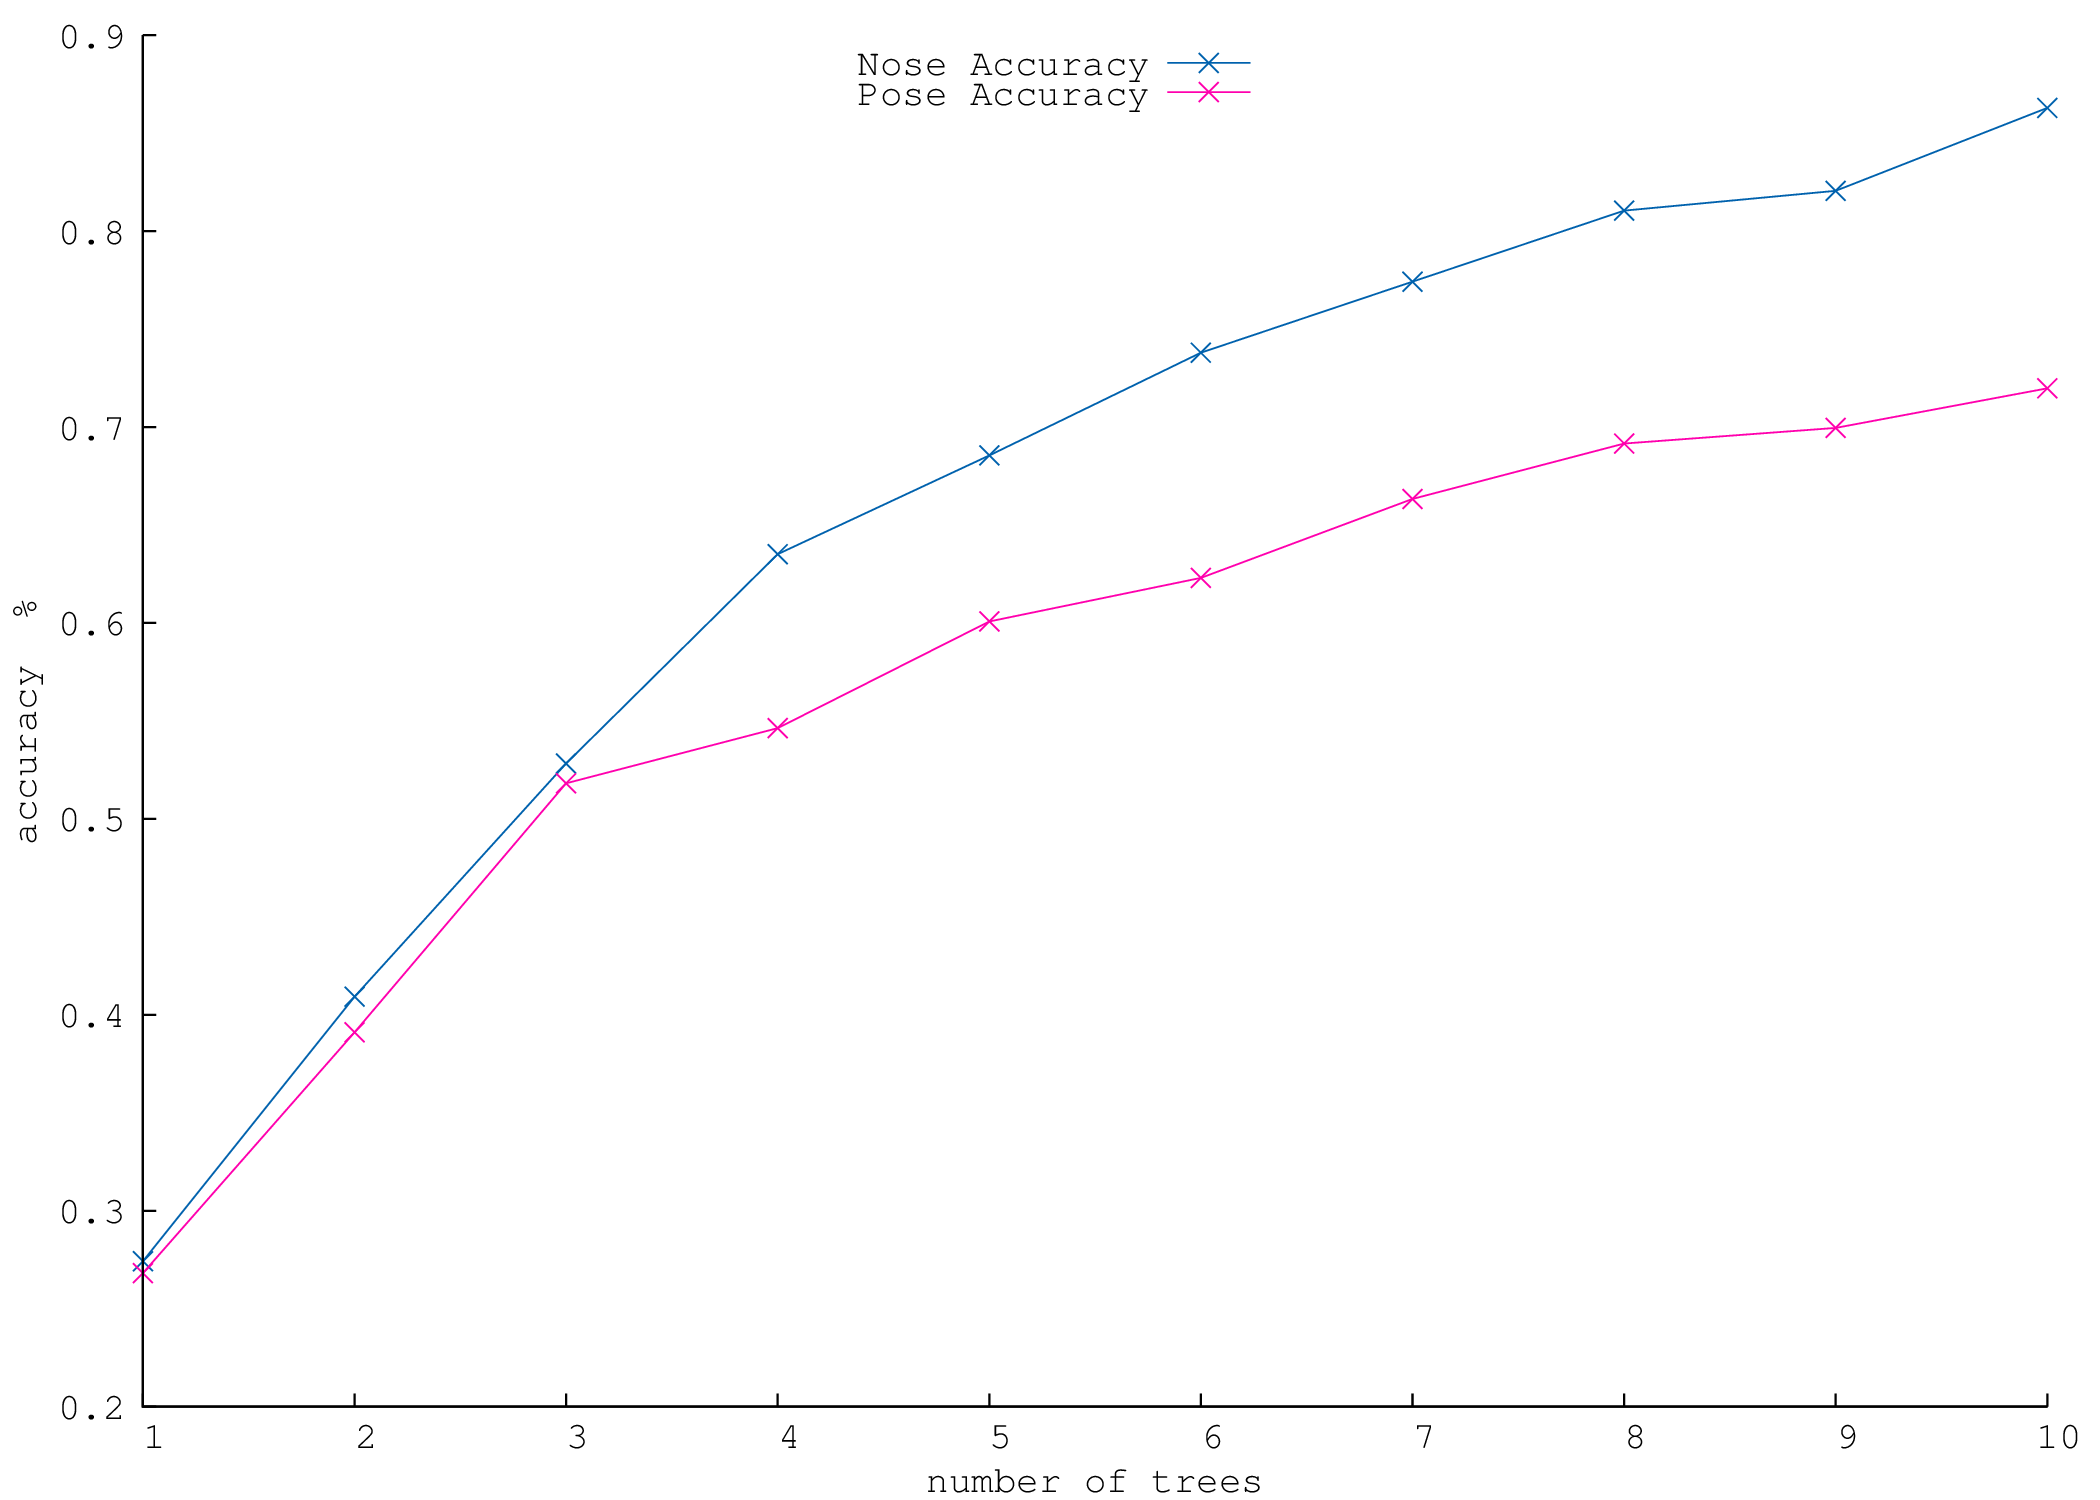
\includegraphics[width=\textwidth]{3daccuracyvstreesstepsize10.png}
                \caption{stride 10}
                \label{fig:naa10}
        \end{subfigure}%
        \caption{accuracy vs number of trees}\label{fig:avt}
\end{figure}


The comparisons between the estimated and ground truth values for Euler angles versus each frame are plotted in figures \ref{fig:pitch}, \ref{fig:yaw}, \ref{fig:roll}. As can be seen from the plots, the overall estimation of yaw and roll angles seems to be better than the pitch angle.

As we increase the tolerance for error, better accuracy can be achieve as can illustrated in figures \ref{fig:noseavse} and \ref{fig:poseavse}. For nose position, the margin of estimated error is extended from 20mm to a range of 15 to 21 mm, the accuracy is increased from below 70\% to over 95\%. Similarly, the accuracy increases from 45\% to 90\% as the margin of error increases from 10 to 20.

\begin{figure}
	\centering
	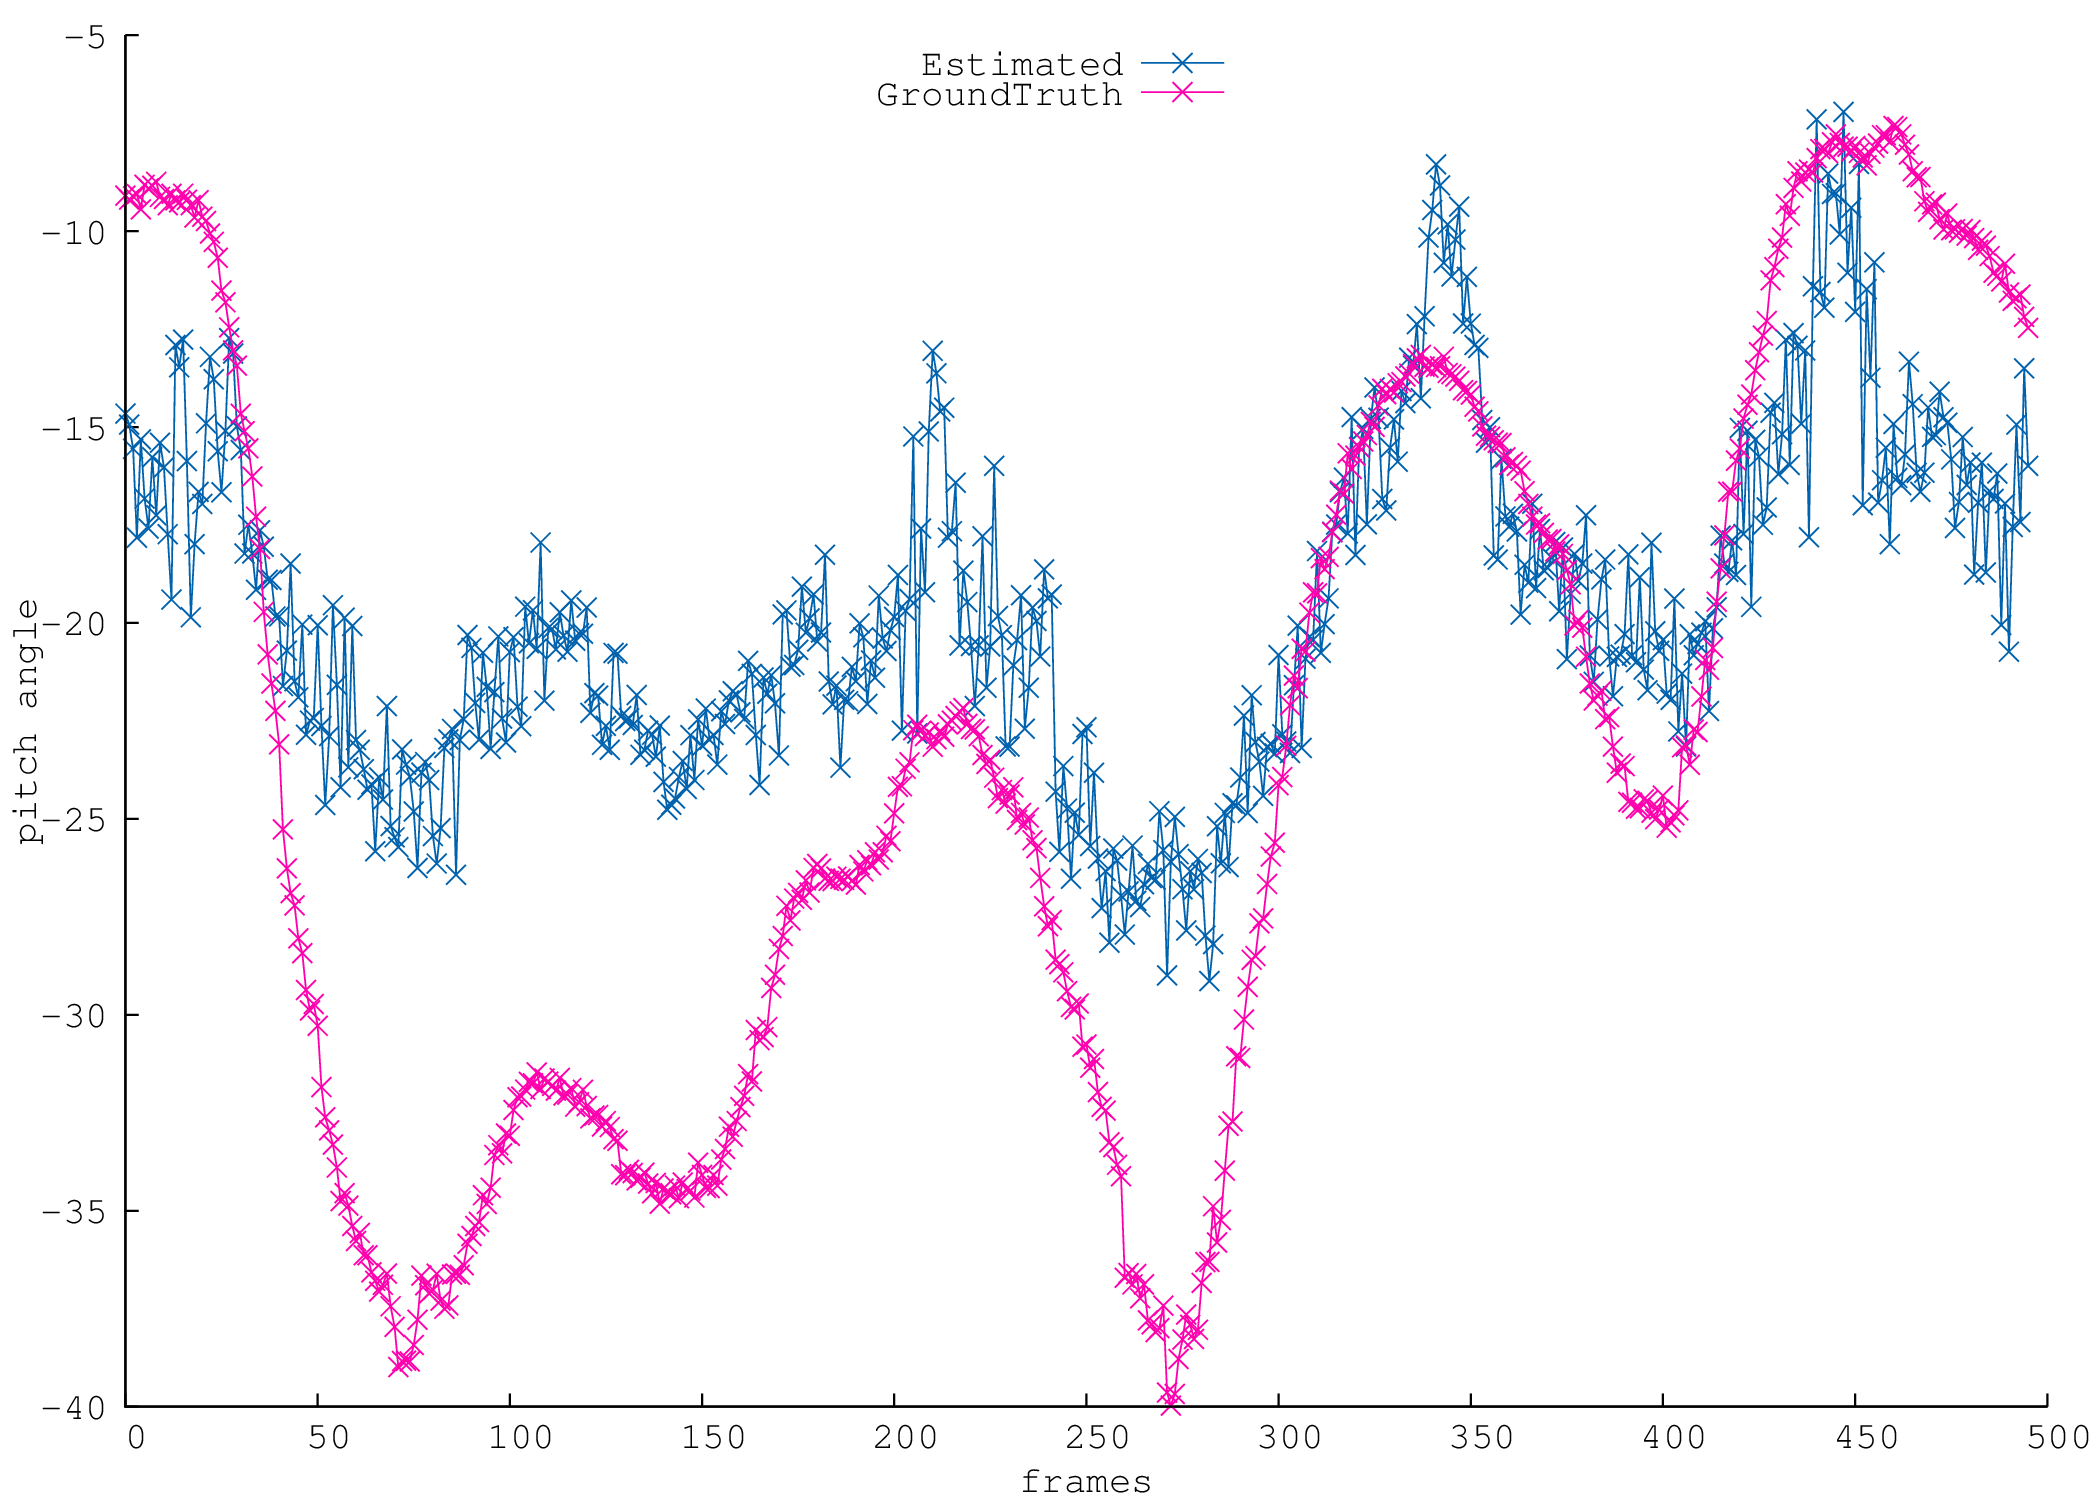
\includegraphics[width=0.8\linewidth]{pitchError5.png}
	\caption[pitch Error]{\label{fig:pitch}}  \textbf{estimated pitch angle and ground truth } 
\end{figure}

\begin{figure}
	\centering
	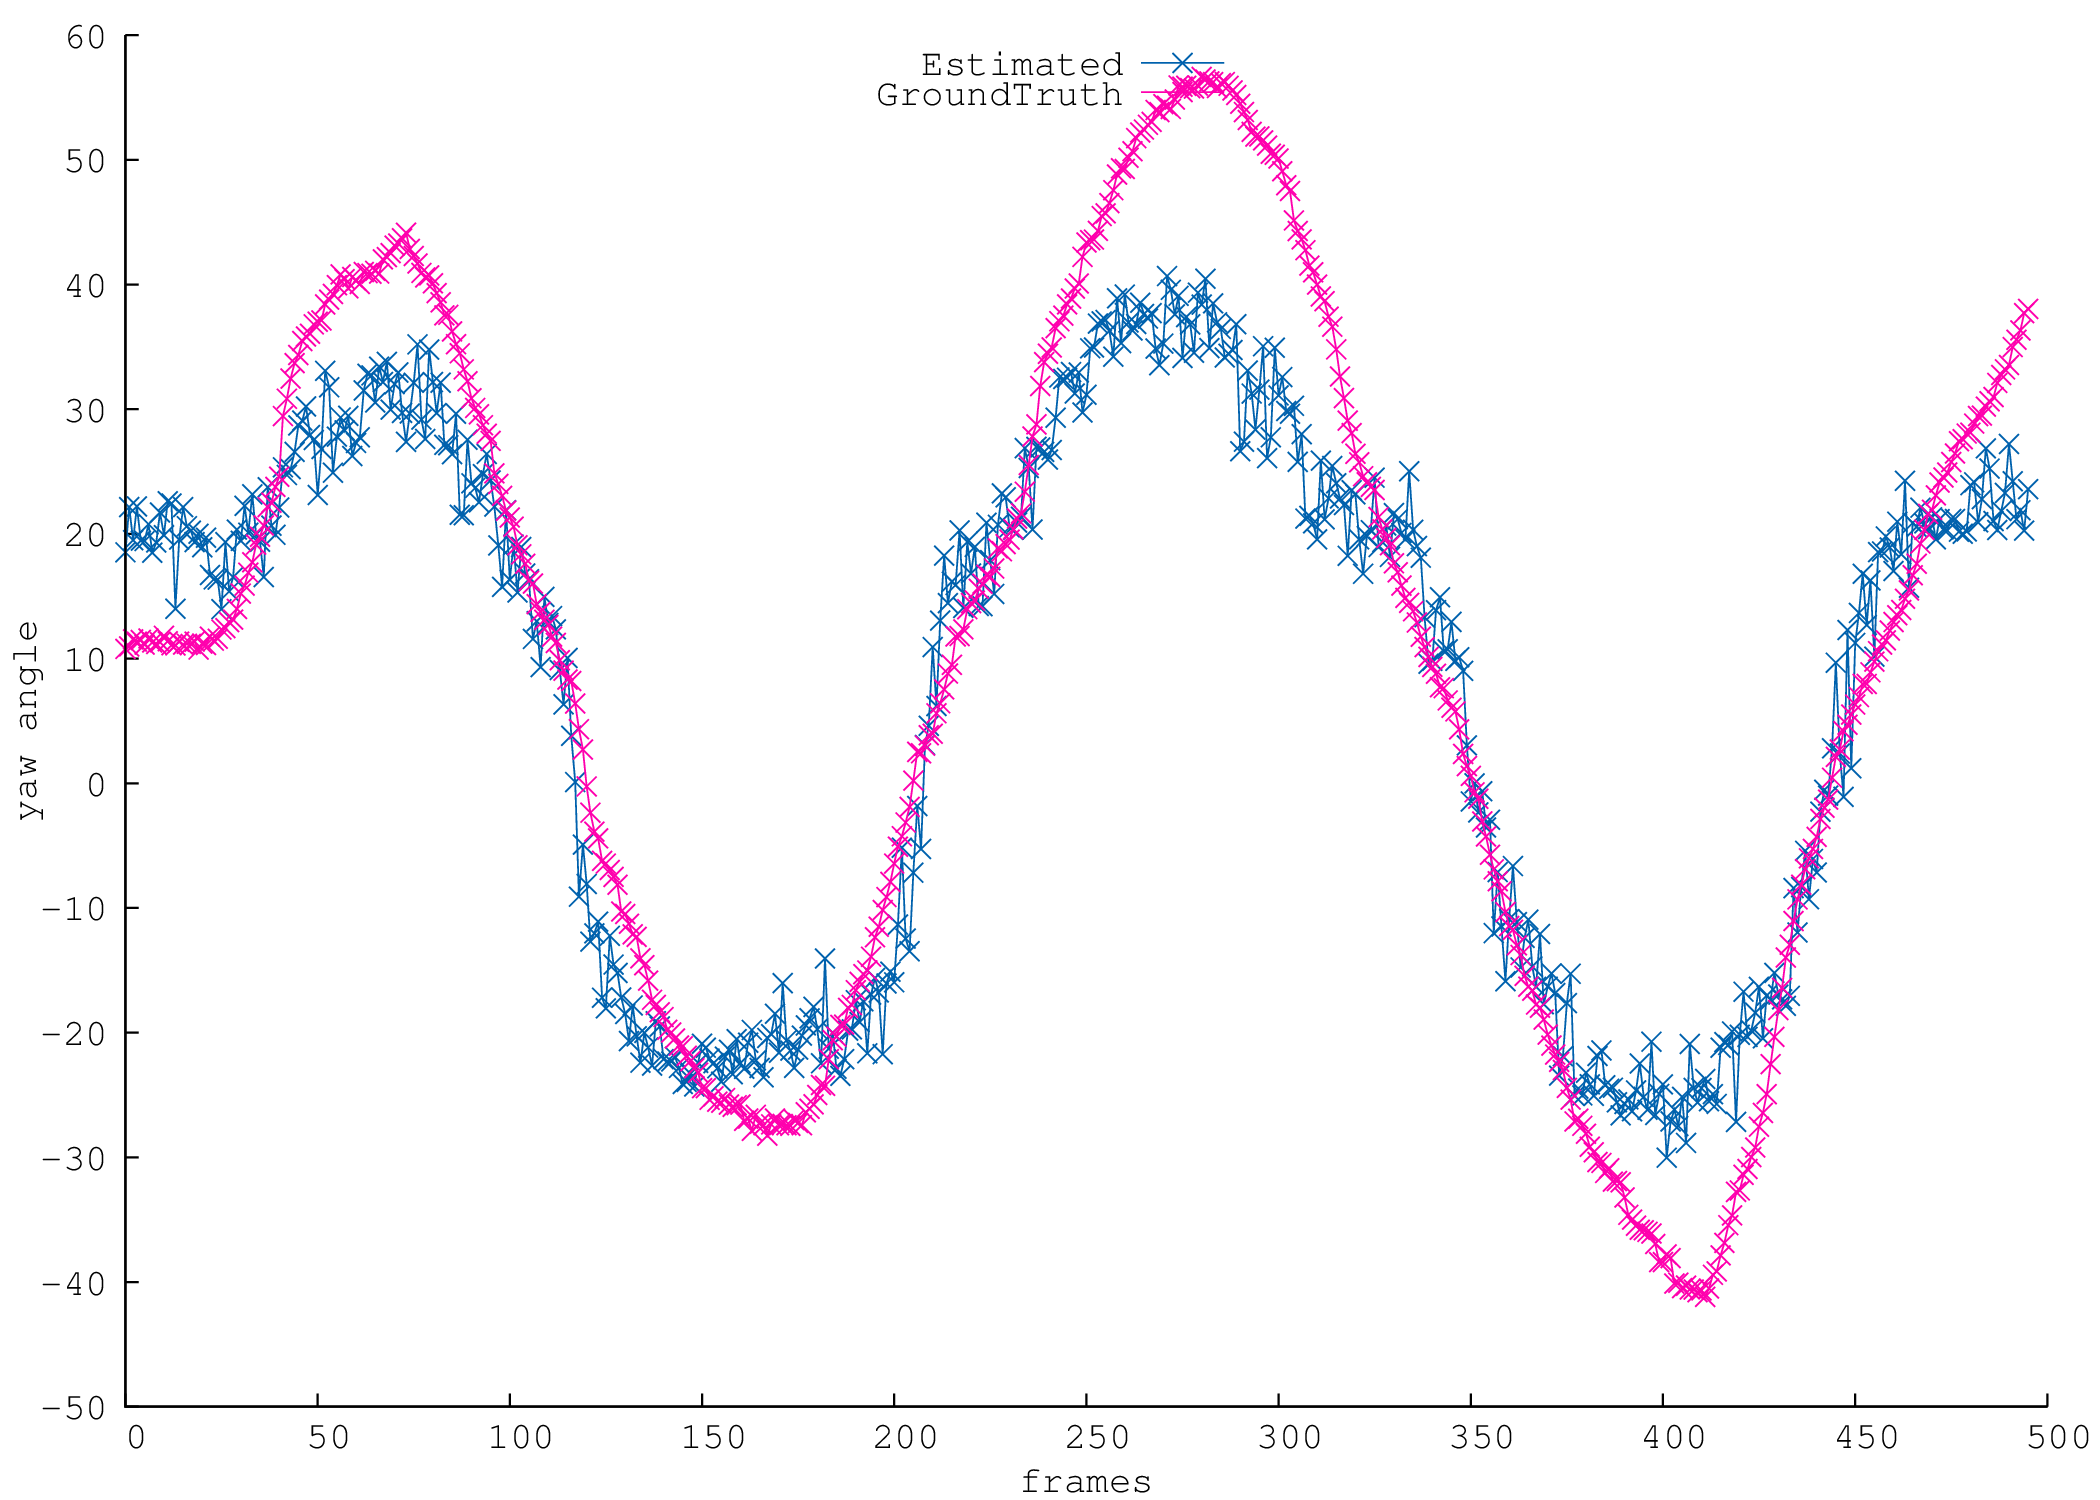
\includegraphics[width=0.8\linewidth]{yawError5.png}
	\caption[yaw Error]{\label{fig:yaw}}  \textbf{estimated yaw angle and ground truth } 
\end{figure}

\begin{figure}
	\centering
	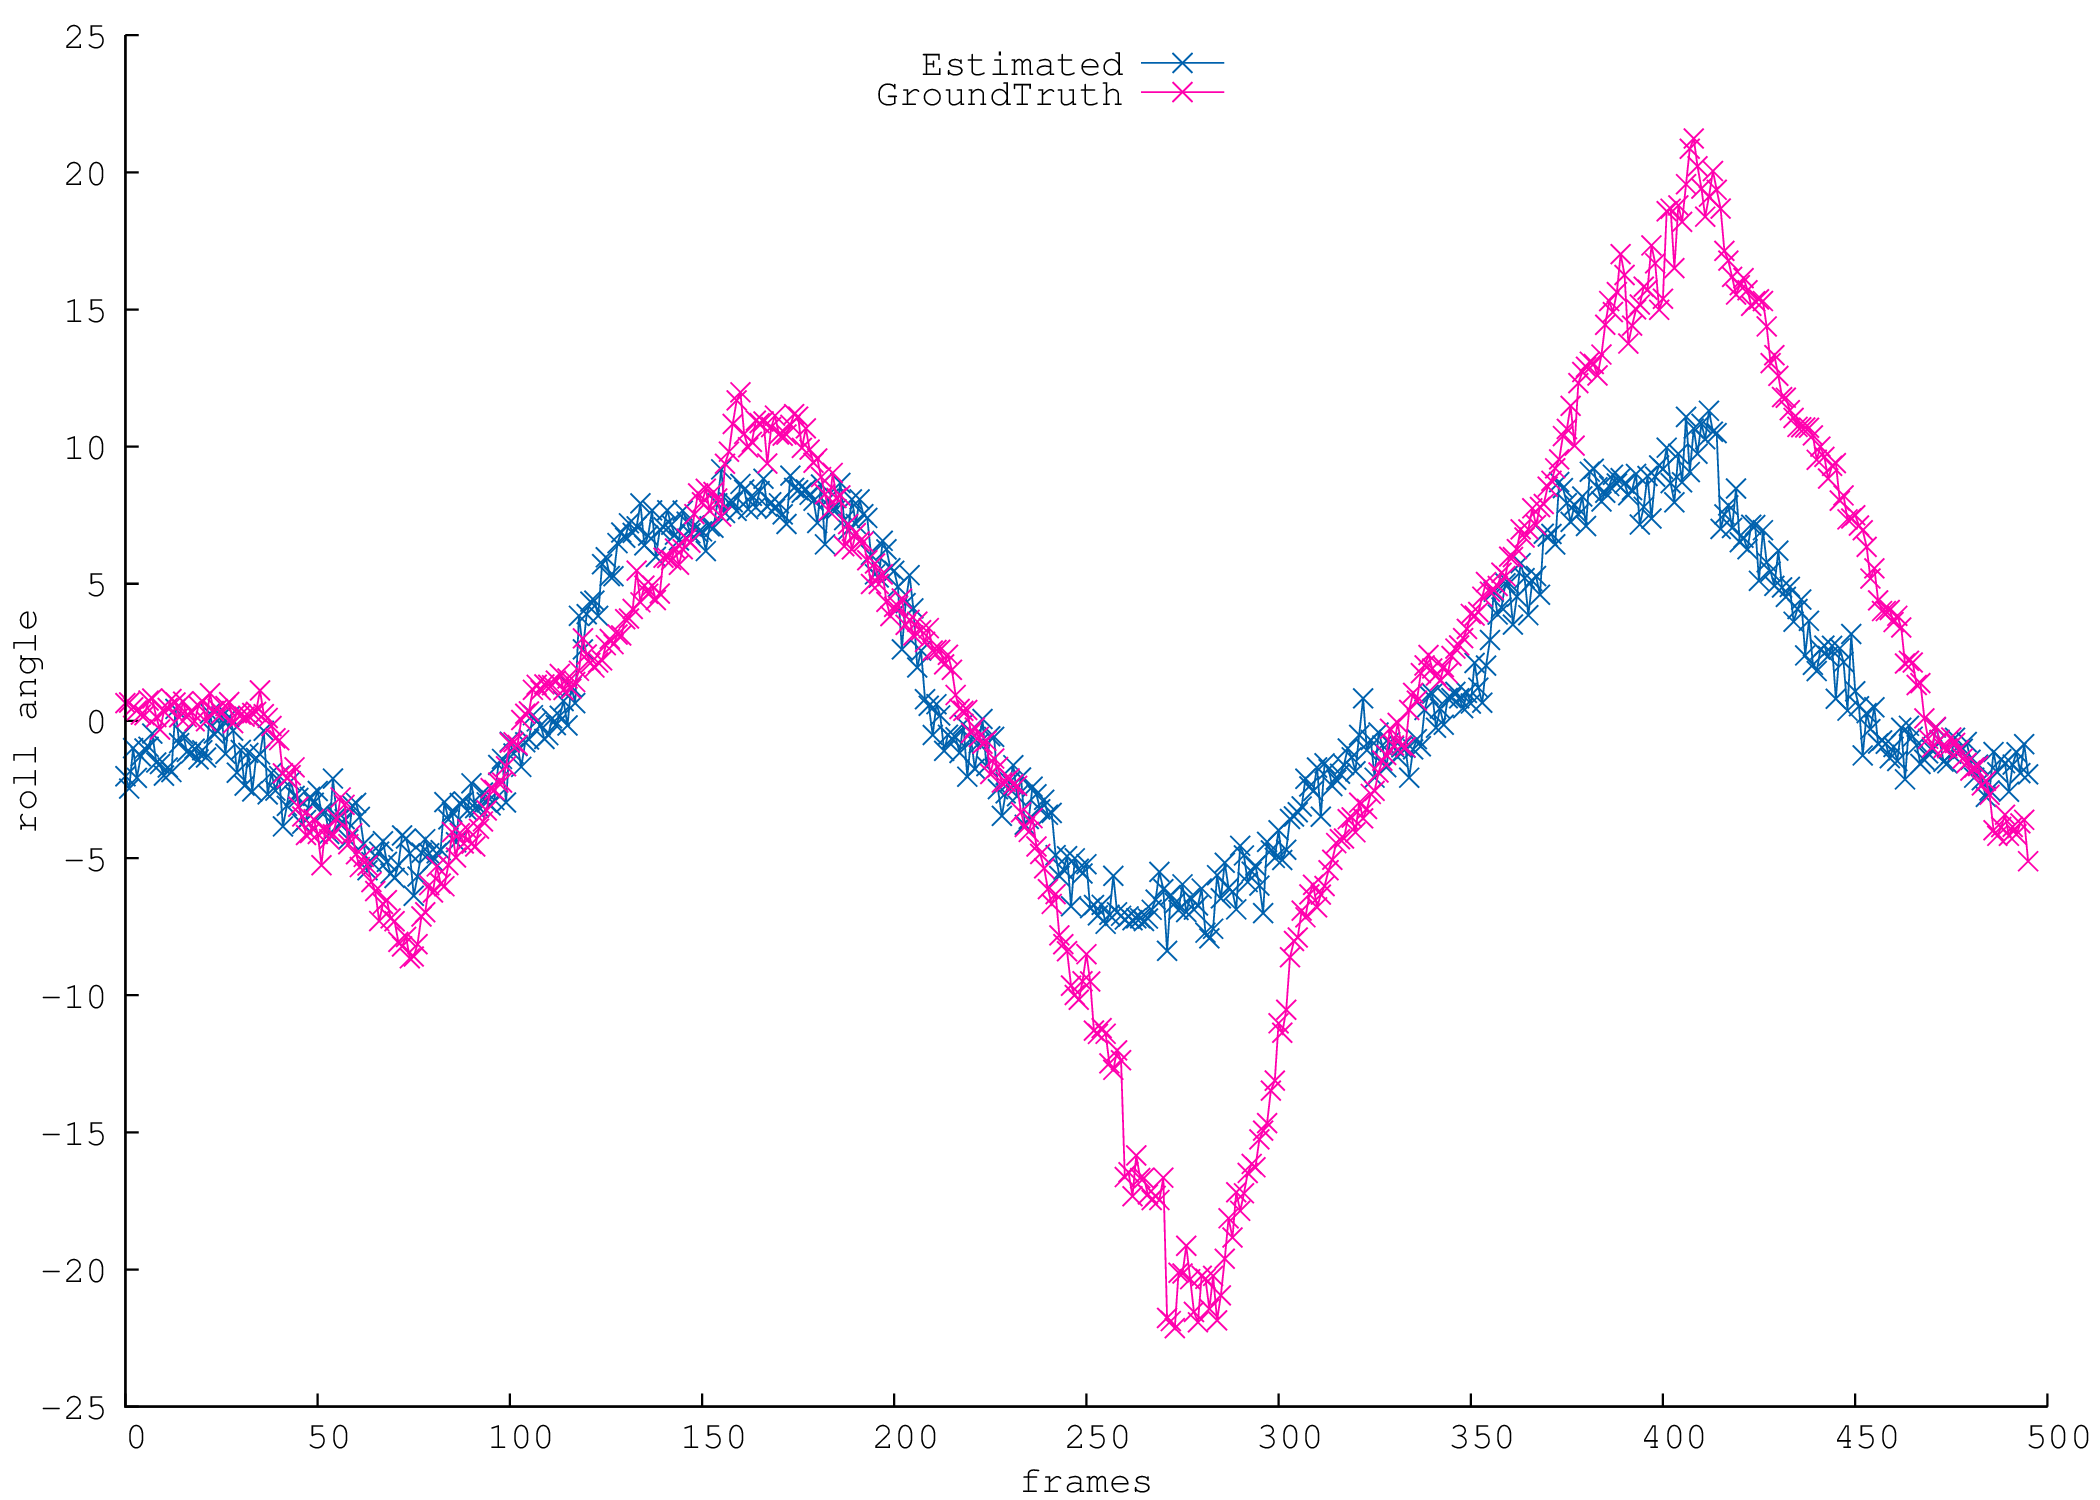
\includegraphics[width=0.8\linewidth]{rollError5.png}
	\caption[roll Error]{\label{fig:roll}}  \textbf{estimated roll angle and ground truth } 
\end{figure}

 

\begin{figure}
	\centering
	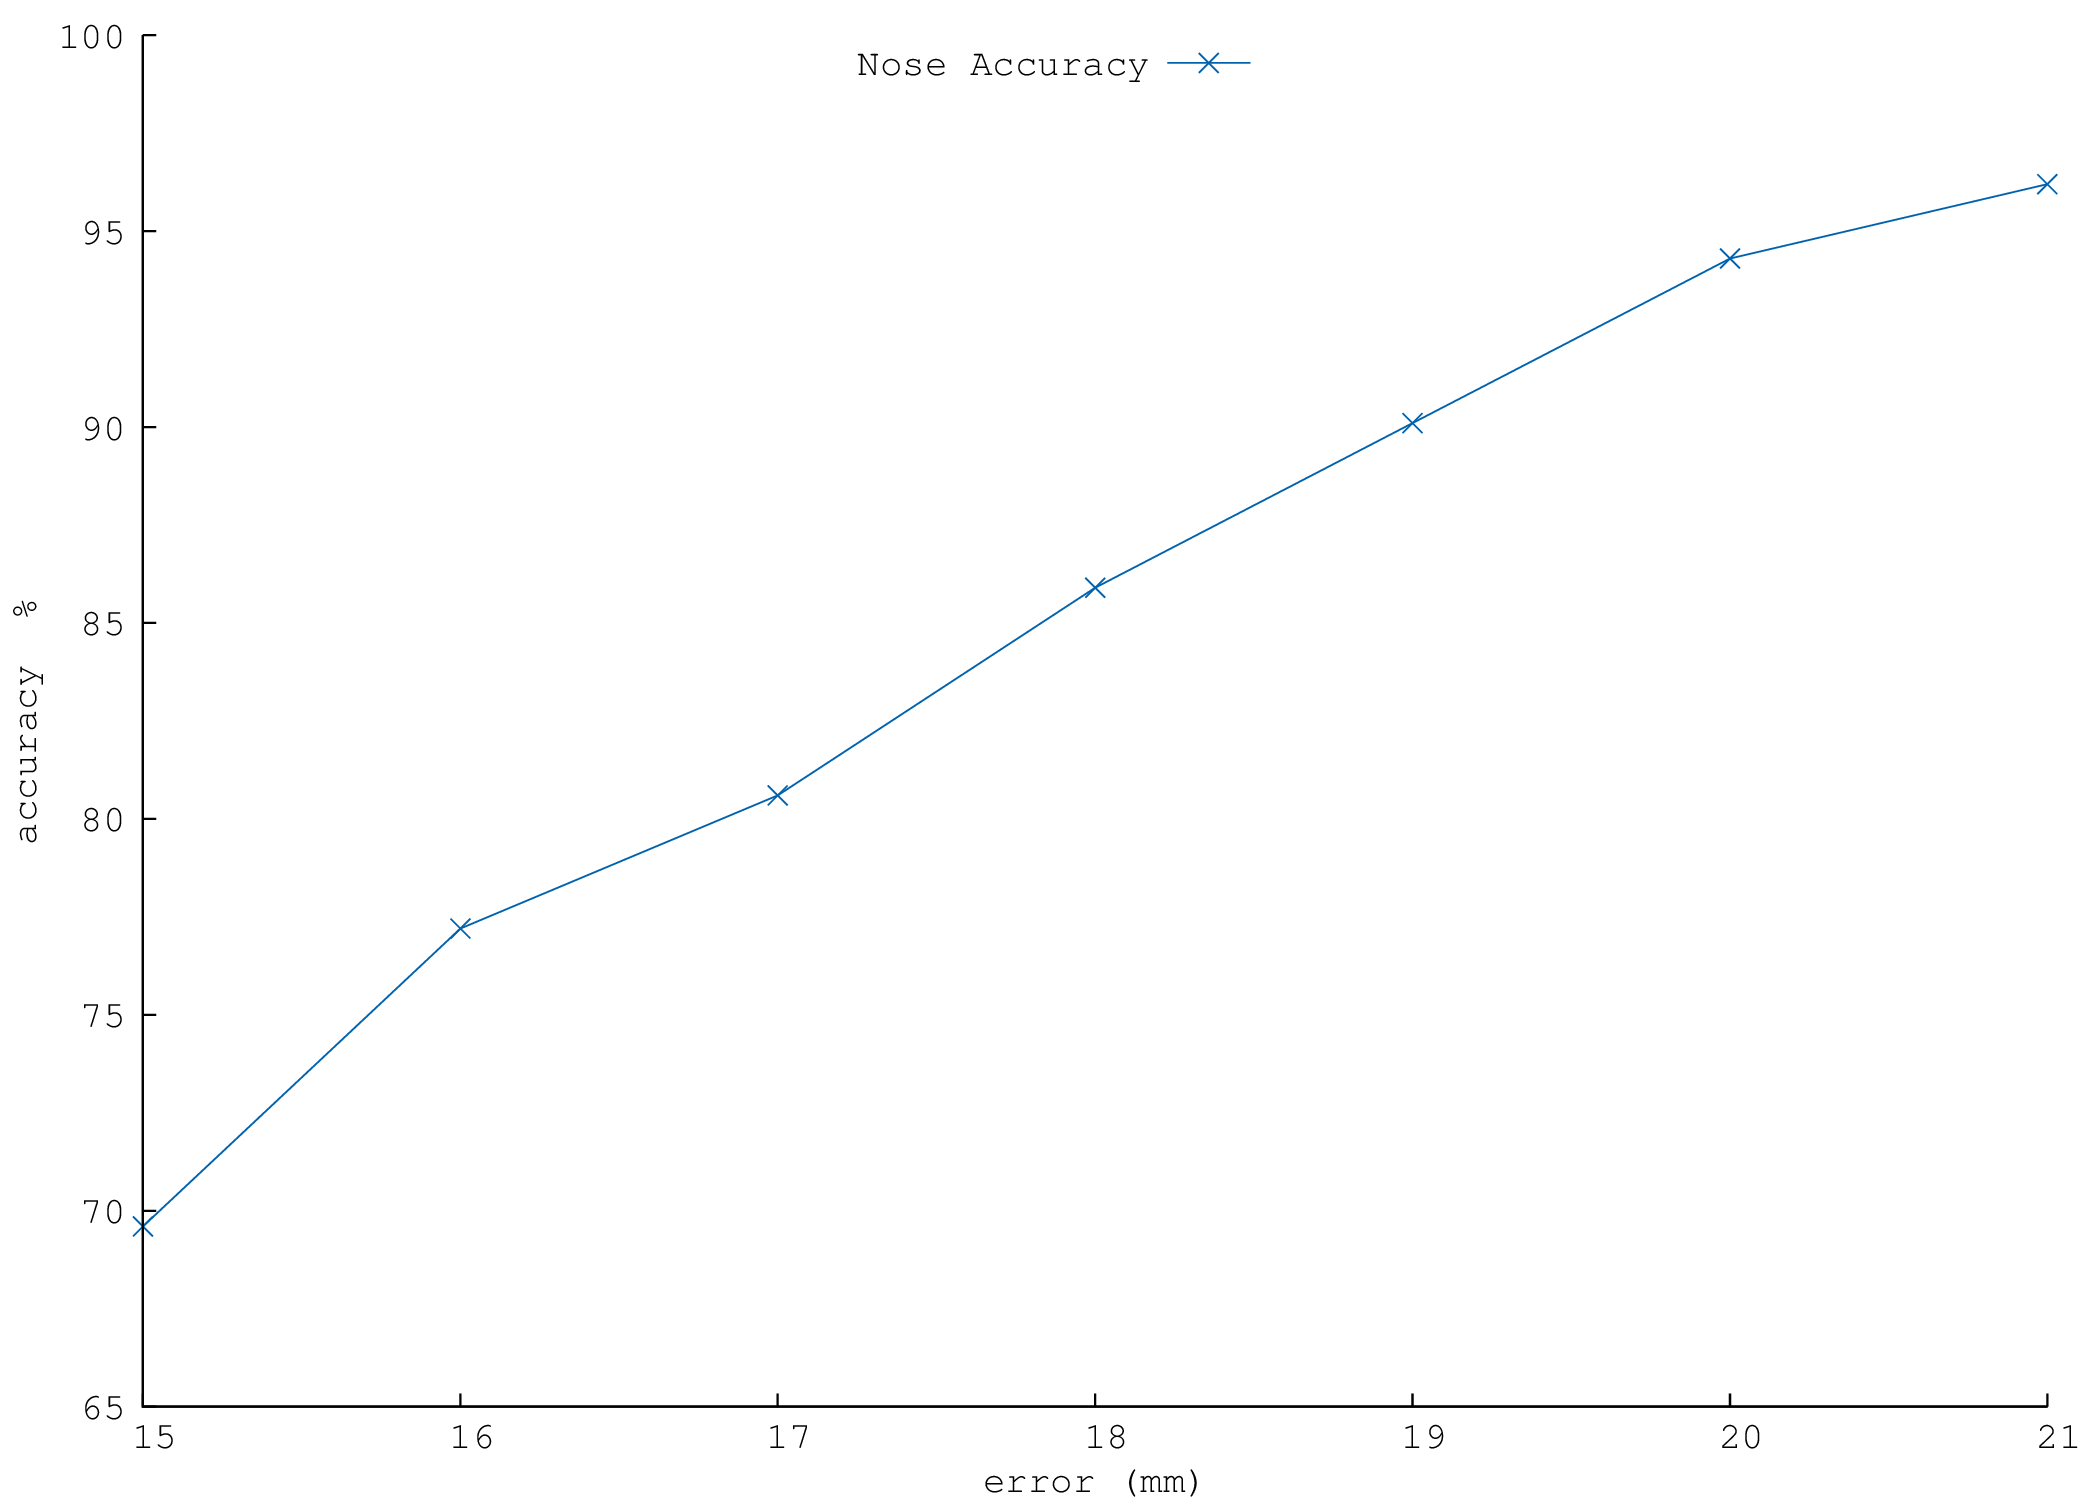
\includegraphics[width=0.8\linewidth]{noseaccuracyvserror.png}
	\caption[Nose accuracy vs error]{\label{fig:noseavse}}  \textbf{nose accuracy vs error stride 5 } 
\end{figure}

\begin{figure}
	\centering
	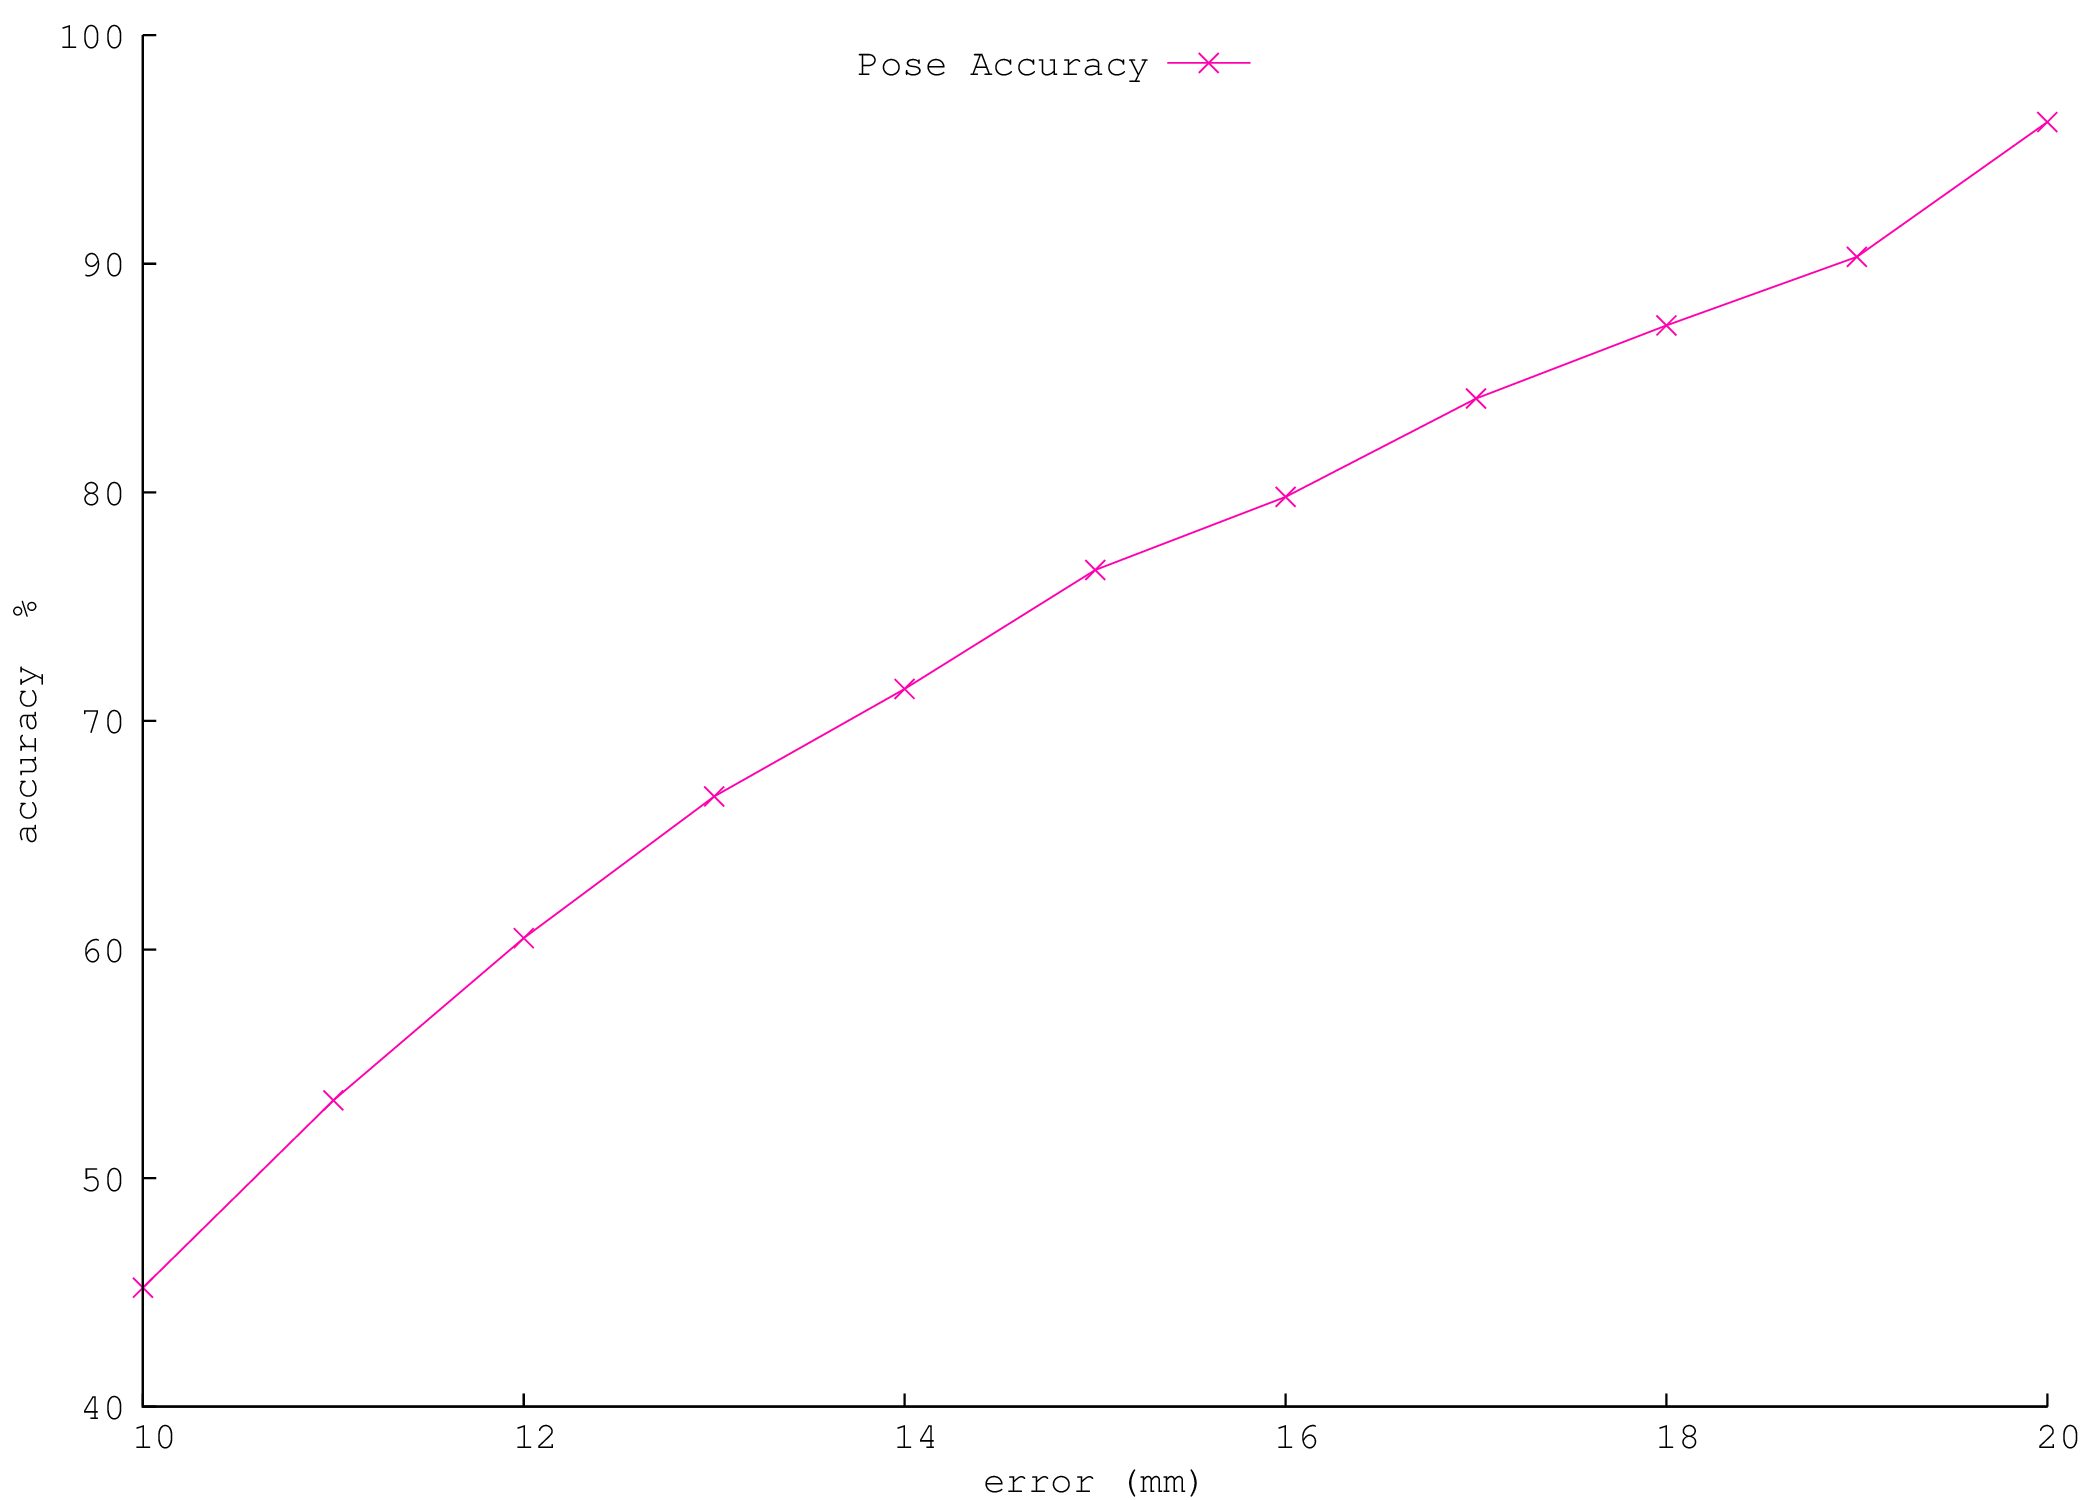
\includegraphics[width=0.8\linewidth]{poseaccuracyvserror.png}
	\caption[Pose accuracy vs error]{\label{fig:poseavse}}  \textbf{pose accuracy vs error stride 5 } 
\end{figure}


